\documentclass{article}[12pt]

     \usepackage{latexsym} % to get LASY symbols
     \usepackage{graphics}
     \usepackage{graphicx} % to insert PostScript figures
     \usepackage{rotating} % for sideways tables/figures
     \usepackage{amsmath}
     \usepackage{amssymb}
     \usepackage[colorlinks=false]{hyperref}
     \usepackage{setspace}
%	     \doublespacing


\usepackage[left=2cm,top=3cm,right=2.5cm,nohead]{geometry}
\def\slantfrac#1#2{\hbox{$\,^{#1}\!/_{#2}$}}

\newcommand{\rf}[1]{\ensuremath{ R_{\mathrm{F}_{#1} } }}
\newcommand{\ldb}{\ensuremath{ \lambda_{\mathrm{th}} }}


\newcommand{\li} {\ensuremath{^{6}}Li\ }

\newcommand{\kb} { \ensuremath{k_{\mathrm{B}}}}

\newcommand{\pli}{\ensuremath{ \mathrm{Li} }}

\newcommand{\TF}{\ensuremath{ T_{F} }}


\begin{document}

\section{Atomic susceptibility}

In the following we want to find what happens with the electric field as it goes through a cloud of atoms.   The approach leads us to think of the atom cloud as a dielectric medium in which the electric field induces a polarization $\vec{\mathcal{P}}(\vec{r}, t)$.   This polarization is a measure of the electric dipole moment per unit volume in the cloud.  If we can calculate the electric dipole moment induced on one atom, $\langle \vec{d} \rangle$, and if we know the density of the cloud, $n(\vec{r})$, then we can simply write the induced polarization as 
\[ \vec{\mathcal{P}}(\vec{r}, t) =  \langle \vec{d} \rangle n(\vec{r}) \]
The induced dipole moment on an atom is proportional to the electric field, and in the more general case the proportionality is given by the electric susceptibility tensor,  $\chi$:
\[ \vec{d} = \epsilon_{0}\chi \vec{E}\]

In cartesian coordinates, one can consider the induced dipole moment along $j$ that results from the perturbation of the atom by the electric field:
\begin{equation}
 \langle\psi(t)| d_{j} | \psi(t) \rangle = \sum_{nm}\gamma_{m}^{*}(t)\gamma_{n}(t) e^{i(E_{m}-E_{n})t/\hbar}\langle m|d_{j}|n\rangle
 \label{eq:dipolemoment}
\end{equation}
where the  electron's wave function is:
\[  | \psi(t)\rangle = \sum_{n}\gamma_{n}(t) e^{-iE_{n}t/\hbar}|n\rangle\]
and the $\gamma$ coefficients satisfy the following equation of motion:
\[ i \hbar \dot{\gamma}_{k}(t) = \sum_{n} \gamma_{n}(t)e^{-i(E_{n}-E_{k})t/\hbar} \langle k | \hat{H}_{\mathrm{int}}(t) | n \rangle \]

The interaction between the atom and the electric field is given by $\hat{H}_{\mathrm{int}}(t)  = -\vec{d}\cdot\vec{E} \cos( \omega t )$.  Since the induced dipole moment depends on a product between $\gamma$ coefficients, it is useful to define the density matrix $\rho_{mn} (t) =  \gamma_{m}^{*}(t)\gamma_{n}(t)$, which has the following equation of motion:
\[ \dot{\rho}_{mn} =- \frac{1}{i\hbar} \sum_{l} \rho_{ln} e^{i(E_{l}-E_{m})t/\hbar} \langle l | \hat{H}_{\mathrm{int}}(t) | m \rangle - \rho_{ml} e^{-i(E_{l}-E_{n})t/\hbar} \langle n | \hat{H}_{\mathrm{int}}(t) | l \rangle \]

It can be seen in Eq.~\ref{eq:dipolemoment}, that the only components of $\rho$ that are of interest are ones which correspond to $m,n$ values that can be coupled by the electric field ($\langle m | d_{j} | n \rangle \neq 0$).  In other words $m,n$ have to be a ground, excited state pair. We can write the equation of motion for such off-diagonal components of the density matrix:
\begin{equation}
\begin{split}
\dot{\rho}_{ge} & =- \frac{1}{i\hbar} \sum_{l} \left( \rho_{le} e^{i(E_{l}-E_{g})t/\hbar} \langle l | \hat{H}_{\mathrm{int}}(t) | g \rangle - \rho_{gl} e^{-i(E_{l}-E_{e})t/\hbar} \langle e | \hat{H}_{\mathrm{int}}(t) | l \rangle \right) \\
 & = - \frac{1}{i\hbar } \sum_{e'}  \rho_{e'e} e^{i(E_{e'}-E_{g})t/\hbar} \langle e' | \hat{H}_{\mathrm{int}}(t) | g \rangle + \frac{1}{i\hbar } \sum_{g'} \rho_{gg'} e^{-i(E_{g'}-E_{e})t/\hbar} \langle e | \hat{H}_{\mathrm{int}}(t) | g' \rangle
\end{split}
\end{equation}
where $e',g'$ index excited states and ground states respectively. 

In doing phase-contrast imaging the probe laser is far off resonance so we can work under the assumption that all the population stays in the ground state of the atom:
\[
\rho_{gg} \approx 1 \ \ \ \  \mathrm{and} \ \ \ \  \rho_{ee'}\approx 0 
\]
which results on equation of motion being simplified to 
\[ \dot{\rho}_{ge} =   \frac{1}{i\hbar } \sum_{g'} e^{-i(E_{g'}-E_{e})t/\hbar} \langle e | \hat{H}_{\mathrm{int}}(t) | g' \rangle \]

We write out explicitly the time dependence of the Hamiltonian
\[ \dot{\rho}_{ge} = -  \frac{1}{i\hbar } \sum_{g'} e^{-i(E_{g'}-E_{e})t/\hbar} \langle e |\vec{d}\cdot\vec{E} | g' \rangle \frac{ e^{i\omega t} + e^{-i\omega t}}{2} \]
and by neglecting the rapidly oscillating terms we get
\[ \dot{\rho}_{ge} = - \frac{1}{2i\hbar } \sum_{g'} e^{-i(E_{g'}-E_{e})t/\hbar-i\omega t} \langle e |\vec{d}\cdot\vec{E} | g' \rangle  \]
This is integrated to obtain
\[ \rho_{ge}(t) =   \frac{1}{2\hbar } \sum_{g'} \frac{e^{i(E_{e}-E_{g'})t/\hbar-i\omega t}}{(E_{e} -E_{g'})/\hbar -\omega   } \langle e |\vec{d}\cdot\vec{E} | g' \rangle  \]
Plugging this back into the expression for the induced dipole moment we obtain
\begin{align}  
\langle d_{j} \rangle & = \sum_{ge}   \frac{1}{2\hbar } \sum_{g'} \frac{e^{i(E_{e}-E_{g'})t/\hbar-i\omega t}}{(E_{e} -E_{g'})/\hbar -\omega   } \langle e |\vec{d}\cdot\vec{E} | g' \rangle  e^{i(E_{g}-E_{e})t/\hbar} \langle e | d_{j} | g \rangle + \mathrm{c.c} \\
& = \frac{1}{2\hbar } \sum_{ge}    \sum_{g'} \frac{e^{i(E_{g}-E_{g'})t/\hbar}}{(E_{e} -E_{g'})/\hbar -\omega   } \langle e |\vec{d}\cdot\vec{E} | g' \rangle   \langle e | d_{j} | g \rangle e^{-i\omega t}  + \mathrm{c.c.} 
\end{align}
We now define the frequency for a transition between $e,g$,  $\omega_{eg} = (E_{e}-E_{g})/\hbar$ and consider the electric field to be constant throughout the extent of the atom's wavefunction so that it can be taken out of the matrix element:
\begin{align}  
\langle d_{j} \rangle & = \sum_{k} \left( \frac{1}{\hbar } \sum_{ge}    \sum_{g'} \frac{e^{i(E_{g}-E_{g'})t/\hbar}}{\omega_{eg} -\omega   } \langle e | d_{k} | g' \rangle   \langle e | d_{j} | g \rangle \right) E_{k} \frac{e^{-i\omega t}}{2}   + \mathrm{c.c.}   \\
& = \epsilon_{0} \sum_{k} \chi_{jk} E_{k} \cos(\omega t)
\end{align}
Notice that we have used the fact that the term in parenthesis is real valued.  The equation above defines the susceptibility tensor of the atom,
\[ \chi_{jk} = \frac{1}{\epsilon_{0}\hbar } \sum_{ge}    \sum_{g'} \frac{e^{i(E_{g}-E_{g'})t/\hbar}}{\omega_{eg} -\omega   } \langle e | d_{k} | g' \rangle   \langle e | d_{j} | g \rangle \]


\section{High field imaging}

At this point it is useful to introduce the states that we are interested in, see Figure~\ref{fig:levels} .
\begin{figure}[h]
\centering 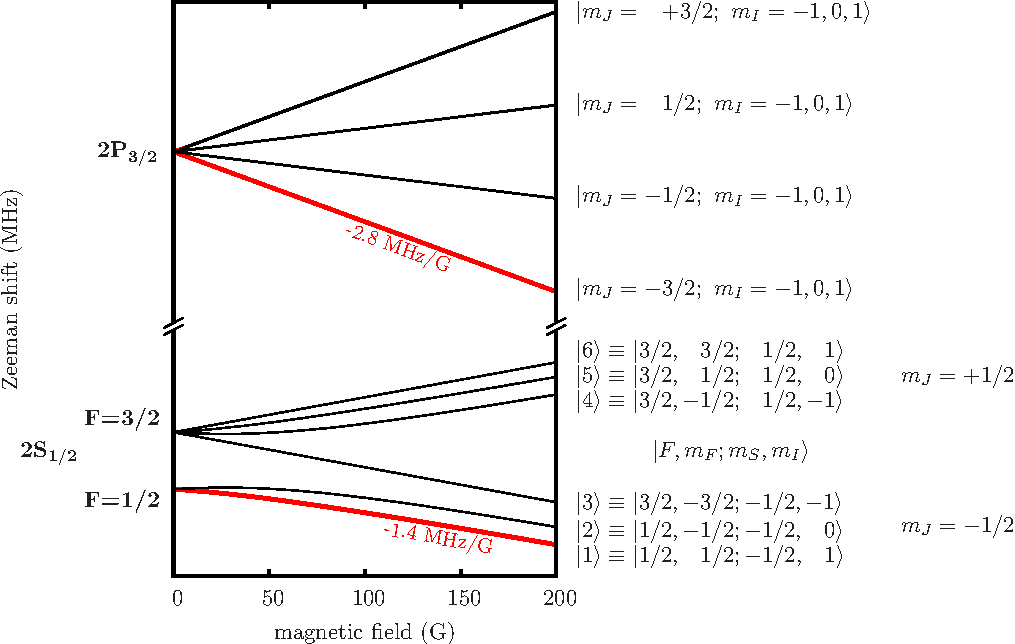
\includegraphics[width=0.85\textwidth]{01eps.pdf}
\caption[Levels relevant for imaging.]{Level diagram relevant for imaging transitions}  \label{fig:levels}
\end{figure}
We are imaging at a high magnetic field, where the nuclear spin is completely decoupled.   We start with atoms in the $m_{J} = -1/2$ level of the 2$S_{1/2}$ ground state and are considering transitions to $m_{J} = -3/2,\,-1/2,\,1/2$ on the 2$P_{3/2}$ excited state.   Since we only have one ground state, the susceptibility tensor is 
\[ \chi_{jk} = \frac{1}{\epsilon_{0}\hbar } \sum_{e}   \frac{ \langle e | d_{k} | g \rangle   \langle e | d_{j} | g \rangle}{\omega_{eg} -\omega   } \]

In our imaging setup the magnetic field is oriented along the $\hat{z}$ axis and the probe beam propagates along $\hat{y}$, perpendicular to the magnetic field.  In this setup the polarization of the light lies on the $xz$ plane.  
The effect of the atoms on the polarization vector of the light is obtained from the index of refraction of the atoms,
\[
  \mathbf{p}_{\mathrm{out}} = \exp\left[ i\frac{\omega }{c}\int (n_{a}(y)-\mathbf{1})dy  \right] \mathbf{p}_{\mathrm{in}} \]
furthermore the index of refraction is just the square root of the electric permittivity, which is the proportionality factor between the electric field and the electric displacement:
\[ \epsilon \vec{E} = \vec{D} = \epsilon_{0}\vec{E} + \vec{\mathcal{P}} = \epsilon_{0}( \mathbf{1} +  \chi n(\vec{r}) )\vec{E}   \]
\[ n_{a}(y) = \sqrt{\epsilon/\epsilon_{0}} = \sqrt{   \mathbf{1} +  \chi n(\vec{r})  } \approx \mathbf{1} + \frac{\chi}{2} n(\vec{r})  \]
this yields,
\[
  \mathbf{p}_{\mathrm{out}} = \exp\left[ i\frac{\omega }{c}\frac{\chi}{2}\int  n(\vec{r})dy  \right]
  \mathbf{p}_{\mathrm{in}} \]
The integral of the density is what we refer to as the column density, $n_{\mathrm{col}}$.   Four our magnetic field orientation and probe propagation direction, the projection of the susceptibility tensor on the $xz$ plane  is a diagonal matrix if expressed on the $\hat{x},\hat{z}$ polarization basis, so if 
\[\mathbf{p}_{\mathrm{in}} = a \hat{x} + b e^{i\gamma} \hat{z} \equiv \left( \begin{array}{c}
a  \\
b e^{i\gamma}    \end{array}   \right)\]
then 
\[
  \mathbf{p}_{\mathrm{out}}  =
    \left( \begin{array}{l}
    \exp\left[ i\frac{\omega }{c}\frac{\chi_{xx}n_{col}}{2}  \right] a  \\
    \exp\left[ i\frac{\omega }{c}\frac{\chi_{zz}n_{col}}{2}  \right]b e^{i\gamma}    \end{array}  \right)
   \]
What this means is that, since in the $\hat{x},\hat{z}$ basis the susceptibility tensor is diagonal, then the polarization components in that basis can be treated independently and each of them acquires a phase shift given by
\begin{align}
\phi_{x} & = \frac{\omega }{c}\frac{\chi_{xx}n_{col}}{2} \\
\phi_{z} & = \frac{\omega }{c}\frac{\chi_{zz}n_{col}}{2} \\
\end{align}

\subsection{Evaluation of the phase shift}

We now proceed to evaluate the diagonal components of the susceptibility tensor, $\chi_{xx}$ and $\chi_{zz}$:
\[ \chi_{xx} = \frac{1}{\epsilon_{0}\hbar } \sum_{e}   \frac{ |\langle e | d_{x} | g \rangle|^{2} }{\omega_{eg} -\omega   } \]
\[ \chi_{zz} = \frac{1}{\epsilon_{0}\hbar } \sum_{e}   \frac{ |\langle e | d_{z} | g \rangle|^{2} }{\omega_{eg} -\omega   } \]
This process boils down to calculating the matrix elements $|\langle e | d_{x} | g \rangle|^{2}$. To do this we have to consider the states that we are dealing with. At high magnetic field the nuclear spin and the total angular momentum of the electron are decoupled and they don't play any role, so the states are 
\begin{align}
|g\rangle & = | R_{g}\, L\,S\,J\,m_{J} \rangle \\
|e\rangle & = | R_{e}\, L\,S\,J\,m_{J} \rangle \\
\end{align}
whre the radial part of the wavefuncion is indicated by $R$.  We evaluate the the matrix element of components of $\vec{d}$ in the spherical basis, $d_{q}$, where $q\in{-1,0,1}$ and then later we can evaluate the cartesian components by projecting them onto the spherical basis vectors.  To evaluate the matrix element, first the Wigner-Eckart theorem\footnote{Sec.~5.4.1 on \cite{edmonds1996angular}} is used to make the angular momentum selection rules explicit in the 3-$j$ symbol.  This defines the reduced matrix element $|\langle R_{e}\, L\,S\,J || d || R_{g}\, L\,S\,J \rangle|^{2}$, 
\begin{align}
|\langle e | d_{q} | g \rangle|^{2} & = \begin{pmatrix} J_{e} & 1 & J_{g} \\ -m_{Je} & q & m_{Jg} \end{pmatrix}^{2}
|\langle R_{e}\, L\,S\,J || d || R_{g}\, L\,S\,J \rangle|^{2}
\end{align}
The dipole moment operator only acts on the electronic angular momentum, $L$, and our quantum state is expressed in the $LS$ coupled scheme, where $L$ and $S$ are coupled to form $J=L+S$.  One can use the formula for the expectation of a single part operator on a coupled scheme\footnote{Sec.~7.1.7 on \cite{edmonds1996angular}}, in this case the dipole moment operating on the $LS$ coupled state. One obtains
\begin{align}
|\langle e | d_{q} | g \rangle|^{2} & = \begin{pmatrix} J_{e} & 1 & J_{g} \\ -m_{Je} & q & m_{Jg} \end{pmatrix}^{2}
(2J_{e}+1)(2J_{g}+1)  \begin{Bmatrix}L_{g} & J_{g} & S \\ J_{e} & L_{e} & 1 \end{Bmatrix}^{2}|\langle R_{e}\, L || d || R_{g}\, L \rangle|^{2}
\end{align}
The fully reduced matrix element can be related to the lifetime, $\tau$, or the natural linewidth, $\Gamma$, of the excited state~\cite{Olivares:98},
\[
|\langle R_{e}\, L || d || R_{g}\, L \rangle|^{2} = \frac{1}{\tau} \frac{ 9\epsilon_{0} \hbar \lambda^{3}}{8 \pi^{2}} = \Gamma\frac{ 9\epsilon_{0} \hbar \lambda^{3}}{8 \pi^{2}} \]
resulting finally in 
\begin{align}
|\langle e | d_{q} | g \rangle|^{2} & = \begin{pmatrix} J_{e} & 1 & J_{g} \\ -m_{Je} & q & m_{Jg} \end{pmatrix}^{2}
(2J_{e}+1)(2J_{g}+1)  \begin{Bmatrix}L_{g} & J_{g} & S \\ J_{e} & L_{e} & 1 \end{Bmatrix}^{2}\Gamma\frac{ 9\epsilon_{0} \hbar \lambda^{3}}{8 \pi^{2}}
\end{align}
At this point we plug in some of the values for our case, $L_{g}=0$, $J_{g} = 1/2$, $m_{Jg}=-1/2$, $L_{e}=1$, and $J_{e}=3/2$.  The $6j$ symbol can be evaluated in Mathematica.  This results in,
\begin{align}
|\langle e | d_{q} | g \rangle|^{2} & = \begin{pmatrix} J_{e} & 1 & J_{g} \\ -m_{Je} & q & m_{Jg} \end{pmatrix}^{2}
\Gamma\frac{ 3\epsilon_{0} \hbar \lambda^{3}}{2 \pi^{2}}
\end{align}
and we can finally write
\begin{align}
|\langle e | d_{i} | g \rangle|^{2} & =  \sum_{q} |\hat{\epsilon}_{i}\cdot \hat{\epsilon}_{q}|^{2} \begin{pmatrix} J_{e} & 1 & J_{g} \\ -m_{Je} & q & m_{Jg} \end{pmatrix}^{2}
\Gamma\frac{ 3\epsilon_{0} \hbar \lambda^{3}}{2 \pi^{2}}
\end{align}
\[ \chi_{xx} = \frac{1}{\epsilon_{0}\hbar } \sum_{e}   \frac{1 }{\omega_{eg} -\omega}  \sum_{q} |\hat{\epsilon}_{x}\cdot \hat{\epsilon}_{q}|^{2} \begin{pmatrix} J_{e} & 1 & J_{g} \\ -m_{Je} & q & m_{Jg} \end{pmatrix}^{2}
\Gamma\frac{ 3\epsilon_{0} \hbar \lambda^{3}}{2 \pi^{2}} \]
\[ \chi_{zz} = \frac{1}{\epsilon_{0}\hbar } \sum_{e}   \frac{1 }{\omega_{eg} -\omega}  \sum_{q} |\hat{\epsilon}_{z}\cdot \hat{\epsilon}_{q}|^{2} \begin{pmatrix} J_{e} & 1 & J_{g} \\ -m_{Je} & q & m_{Jg} \end{pmatrix}^{2}
\Gamma\frac{ 3\epsilon_{0} \hbar \lambda^{3}}{2 \pi^{2}} \]
If we label our possible excited states as $e\in\{\sigma_{-}, \pi, \sigma_{+}\}$ then we have
\begin{align}
\chi_{xx} & = \Gamma\frac{ 3\lambda^{3}}{2 \pi^{2}} \left(   \frac{1 }{\omega_{\sigma_{-}g} -\omega}  |\hat{\epsilon}_{x}\cdot \hat{\epsilon}_{-}|^{2} \begin{pmatrix} 3/2 & 1 & 1/2 \\ 3/2 & -1 & -1/2 \end{pmatrix}^{2} 
+ \frac{1 }{\omega_{\sigma_{+}g} -\omega}  |\hat{\epsilon}_{x}\cdot \hat{\epsilon}_{+}|^{2} \begin{pmatrix} 3/2 & 1 & -1/2 \\ 1/2 & +1 & -1/2 \end{pmatrix}^{2} \right) \\
 \chi_{zz} & = \Gamma\frac{ 3  \lambda^{3}}{2 \pi^{2}}     \frac{1 }{\omega_{\pi g} -\omega}   |\hat{\epsilon}_{z}\cdot \hat{\epsilon}_{0}|^{2} \begin{pmatrix} 3/2 & 1 & 1/2 \\ 1/2 & 0 & -1/2 \end{pmatrix}^{2}
\end{align}
The unit vector projections and $3j$-symbols are evaluated to give
\begin{align}
\chi_{xx} & = \Gamma\frac{ 3 \lambda^{3}}{2 \pi^{2}} \left(   \frac{1 }{\omega_{\sigma_{-}g} -\omega}  \frac{1}{8} 
+ \frac{1 }{\omega_{\sigma_{+}g} -\omega} \frac{1}{24} \right)  
= - \frac{ 3\epsilon_{0} \lambda^{3}}{2 \pi^{2}} \left(   \frac{1 }{\Delta_{-}}  \frac{1}{8} + \frac{1 }{\Delta_{+}} \frac{1}{24}  \right) \\
 \chi_{zz} & = \Gamma\frac{ 3  \lambda^{3}}{2 \pi^{2}}     \frac{1 }{\omega_{\pi g} -\omega}    \frac{1}{6}
  = -\frac{ 3\epsilon_{0}  \lambda^{3}}{2 \pi^{2}}     \frac{1 }{\Delta_{\pi}}    \frac{1}{6}
\end{align}
where we have introduced $\Delta$, the detuning of the probe beam with respect to the excited state in units of the linewidth.  The phase-shifts are then:
\begin{align}
\phi_{x} & = -\frac{\omega }{c}\frac{n_{col}}{2} \frac{ 3 \lambda^{3}}{2 \pi^{2}} \left(   \frac{1 }{\Delta_{-}}  \frac{1}{8} + \frac{1 }{\Delta_{+}} \frac{1}{24}  \right) \\
\phi_{z} & = - \frac{\omega }{c}\frac{n_{col}}{2} \frac{ 3  \lambda^{3}}{2 \pi^{2}}     \frac{1 }{\Delta_{\pi}}    \frac{1}{6} 
\end{align}
and replacing $\omega/c = 2\pi/\lambda$
\begin{align}
\phi_{x} & = -n_{col} \frac{ 3 \lambda^{2}}{2 \pi} \left(   \frac{1 }{\Delta_{-}}  \frac{1}{8} + \frac{1 }{\Delta_{+}} \frac{1}{24}  \right) \\
\phi_{z} & = -n_{col} \frac{ 3  \lambda^{2}}{2 \pi}     \frac{1 }{\Delta_{\pi}}    \frac{1}{6} 
\end{align}
If one introduces the maximal cross section $\sigma = 3\lambda^{2} /(2\pi)$ and the effective cross sections
\[
 \sigma_{iq} =   \sigma (2 J_{e} + 1) \sum_{q} |\hat{\epsilon}_{i}\cdot \hat{\epsilon}_{q}|^{2} \begin{pmatrix} J_{e} & 1 & J_{g} \\ -m_{Je} & q & m_{Jg} \end{pmatrix}^{2} \]
then the phase shifts can be written as 
\begin{align}
\phi_{x} & = -n_{col}  \left(   \frac{\sigma_{x-} }{4\Delta_{-}}  + \frac{\sigma_{x+} }{4\Delta_{+}} \right) \\
\phi_{z} & = -n_{col} \frac{\sigma_{z\pi} }{4\Delta_{\pi}}   
\end{align}

\subsection{ Lorentzian lineshape for smaller detunings}

In the above treatment we have neglected any absorption of light by the atoms (the susceptibiliy that was derived is a real valued  quantity) and we also have neglected saturation effects.  In this section we outline an attempt to consider these two effects.  Even though the stuff presented in this section sort of makes sense, no rigorous derivations have been made.  It is recommended that when in doubt just go a few linewidths away from resonance so that absorption and saturation are negligible and the phase shift formulas described above are directly applicable. 

When absorption and saturation are considered, the imaginary part of the susceptibility gives rise to attenuation of the probe beam by a factor of $e^{-\alpha}$, where $\alpha$ has a power broadened lorentzian profile of width $\Gamma\sqrt{1 + 2 I/ I_{\mathrm{sat}}}$.    The attenuation, $\alpha$, and the phase shift are related to one another by $\phi = -\Delta\alpha$.  In our case, each of the $\hat{x}$ and $\hat{z}$ polarization is attenuated with $\alpha$ given by
\begin{align}
\alpha_{x} & = n_{col}  \left(   \frac{\sigma_{x-} }{1+4\Delta_{-}^{2} + 2I_{x}/I_{\mathrm{sat,x}}}  + \frac{\sigma_{x+} }{1+4\Delta_{+}^{2} + 2I_{x}/I_{\mathrm{sat,x}}} \right) \\
\alpha_{z} & = n_{col} \frac{\sigma_{z\pi} }{1+4\Delta_{\pi}^{2} + 2I_{z}/I_{\mathrm{sat,z}}}   
\end{align}
Here, 
\[ I_{\mathrm{sat},i} = \hbar\omega\Gamma /\left( \sum_{q} \sigma_{iq} \right) \]
and,  for a polarization input given by $( a ,\, be^{i\gamma}$,  

\bibliographystyle{osa}
\bibliography{pmd}

\end{document}